\documentclass[]{article}
\usepackage{lmodern}
\usepackage{amssymb,amsmath}
\usepackage{ifxetex,ifluatex}
\usepackage{fixltx2e} % provides \textsubscript
\ifnum 0\ifxetex 1\fi\ifluatex 1\fi=0 % if pdftex
  \usepackage[T1]{fontenc}
  \usepackage[utf8]{inputenc}
\else % if luatex or xelatex
  \ifxetex
    \usepackage{mathspec}
  \else
    \usepackage{fontspec}
  \fi
  \defaultfontfeatures{Ligatures=TeX,Scale=MatchLowercase}
\fi
% use upquote if available, for straight quotes in verbatim environments
\IfFileExists{upquote.sty}{\usepackage{upquote}}{}
% use microtype if available
\IfFileExists{microtype.sty}{%
\usepackage{microtype}
\UseMicrotypeSet[protrusion]{basicmath} % disable protrusion for tt fonts
}{}
\usepackage[unicode=true]{hyperref}
\hypersetup{
            pdfborder={0 0 0},
            breaklinks=true}
\urlstyle{same}  % don't use monospace font for urls
\usepackage{graphicx,grffile}
\makeatletter
\def\maxwidth{\ifdim\Gin@nat@width>\linewidth\linewidth\else\Gin@nat@width\fi}
\def\maxheight{\ifdim\Gin@nat@height>\textheight\textheight\else\Gin@nat@height\fi}
\makeatother
% Scale images if necessary, so that they will not overflow the page
% margins by default, and it is still possible to overwrite the defaults
% using explicit options in \includegraphics[width, height, ...]{}
\setkeys{Gin}{width=\maxwidth,height=\maxheight,keepaspectratio}
\IfFileExists{parskip.sty}{%
\usepackage{parskip}
}{% else
\setlength{\parindent}{0pt}
\setlength{\parskip}{6pt plus 2pt minus 1pt}
}
\setlength{\emergencystretch}{3em}  % prevent overfull lines
\providecommand{\tightlist}{%
  \setlength{\itemsep}{0pt}\setlength{\parskip}{0pt}}
\setcounter{secnumdepth}{0}
% Redefines (sub)paragraphs to behave more like sections
\ifx\paragraph\undefined\else
\let\oldparagraph\paragraph
\renewcommand{\paragraph}[1]{\oldparagraph{#1}\mbox{}}
\fi
\ifx\subparagraph\undefined\else
\let\oldsubparagraph\subparagraph
\renewcommand{\subparagraph}[1]{\oldsubparagraph{#1}\mbox{}}
\fi

% set default figure placement to htbp
\makeatletter
\def\fps@figure{htbp}
\makeatother


\date{}

\begin{document}

~~~~~~~~~~~~~~~~~~~~~~~~~~~~~~~~~~~~~~~~~~~~~~~~~~~~~~~~~~~~~~~~~~~~~~~~~~
Data:9/1/2017

~~~~~~~~~~~~~~~~~~~~~~~~~~~~~~~~~~~~~~~~~~~~~~~~~~~~~~~~~~~~~~~~~~~~~~~~~~
Docente: Carlo Signorelli

~~~~~~~~~~~~~~~~~~~~~~~~~~~~~~~~~~~~~~~~~~~~~~~~~~~~~~~~~~~~~~~~~~~~~~~~~~
Lezione: incidenti e infortuni

~~~~~~~~~~~~~~~~~~~~~~~~~~~~~~~~~~~~~~~~~~~~~~~~~~~~~~~~~~~~~~~~~~~~~~~~~~
Sbobinatore Morisi Niccolò

~

Caso del mese: Emergenza meningite (paragrafo)

Il titolo del Corriere della sera è emblematico: ``la meningite non è
una emergenza ma fa paura''; infatti i dati 2014-2015-2016 sottolineano
come ci sia una stabilità del fenomeno meningite ma fa paura per i 629
morti su 6786 casi, ossia un 10\%, e di fatto è uno dei tassi di
letalità più alti tra le malattie infettive in circolazione. I casi di
meningite sono legati diversi agenti infettivi e ricordando i maggiori
brevemente meningococco con tutti i siero gruppi, pneumococco e alcune
meningite virali che sono comunemente meno gravi. La vaccinazione può
essere utile in quelle da meningococco di gruppo B, con maggior
incidenza nel primo anno di vita e del gruppo C, con una incidenza che
aumenta dal secondo anno di vita ed è quella che ha causato anche
qualche morto in età adolescenziale e adulta. La situazione attuale di
copertura immunitaria è determinata dal fatto che dal 2012 tutti i
bambini a 13 mesi dovrebbero aver fatto il meningogocco C, purtroppo
però questa vaccinazione è iniziata a macchia di leopardo tra il 2016 e
il 2012 nelle diverse regioni e quindi per i bambini nati prima del 2012
non si ha la certezza della copertura vaccinale, soprattutto per
Lombardia e Piemonte che sono state le ultime ad attivarla. Questa
vaccinazione in linea teorica è a lungo termine ma il quanto lungo non
si sa con certezza, quindi in adolescenza (11-13 anni) c'è il consiglio
di fare un richiamo che rinforzi l'immunità di chi aveva già fatto il
vaccino e crrei immunità dove questa manca. La vaccinazione è
raccomandata e gratuita anche per le categoria a rischio ossia i malati
cronici e i frequentatori di comunità chiuse. In altre situazioni non ci
sono indicazioni anche se in questo periodo le richieste di vaccino sono
aumentate del 130\% nel mese di Dicembre e questo è dovuto alla reazione
emotiva alle notizie trasmesse dai media che chiaramente deve essere
gestita dalla Sanità Pubblica. Per quanto riguarda la vaccinazione per
il meningocco B invece oggi è applicata solo in Toscana ma diventerà
nazionale con i nuovi LEA ancora in via di approvazione.

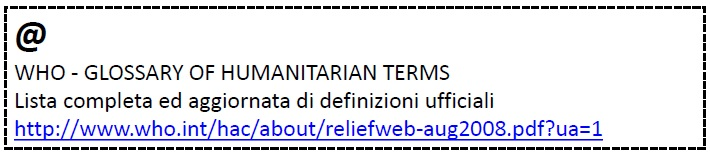
\includegraphics[width=4.76806in,height=3.47639in]{media/image1.emf}

Incidenti ed infortuni(Sezione)

In questa sezione si discuterà di incidenti stradali, e infortuni, sia
domestici che sul lavoro. Questo però ha come preambolo le leggi e i
regolamenti, strumenti che se applicati correttamente dovrebbero
prevenire qualsiasi incidente o infortunio.

Legge e regolamenti(Sottosezione)

Le leggi e i regolamenti sono strumenti molto utilizzati dalla Sanità
Pubblica anche se non è l'unico. Una cosa particolare è che le leggi
sono il riflesso della società e delle coscienze al momento della loro
emanazione e quindi un tempo c'erano le misure di contumacia e
quarantena mentre oggi ci sono norme di tutela ambientale, di sicurezza
sul lavoro e il codice della strada. Quindi se una volta prevalevano le
azioni obbligatorie di Polizia Sanitaria, oggi siamo nell'era delle
notifiche e della sorveglianza, accompagnate comunque da norme ma a più
ampio respiro.

Questi sono due schemi che raccolgono le norme più importanti in Italia
e gli atti più incisivi nel mondo.

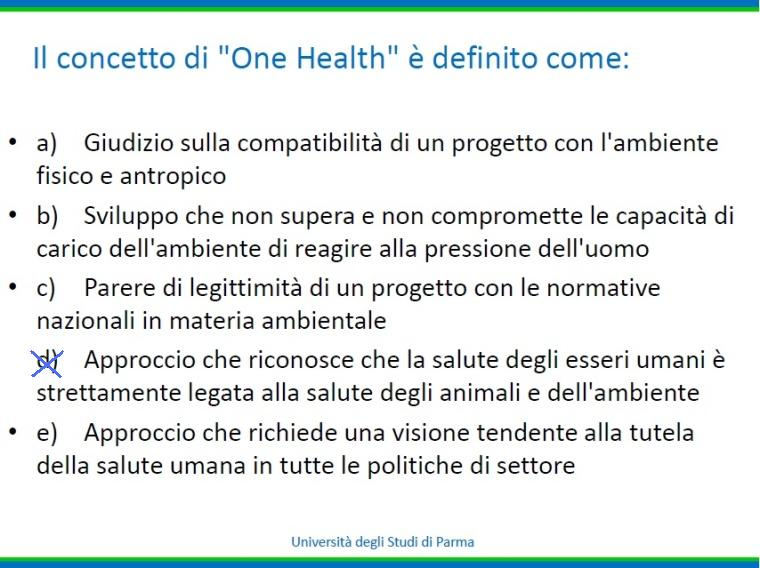
\includegraphics[width=4.53611in,height=2.89931in]{media/image2.emf}

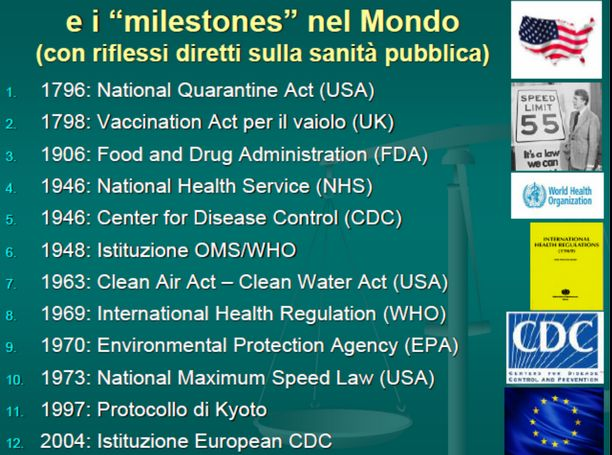
\includegraphics[width=4.63472in,height=3.18611in]{media/image3.emf}Incidenti
stradali (Sottosezione)

Definizione

Si definisce come incidente stradale \emph{un incidente avvenuto in una
strada aperta alla circolazione pubblica, con una o più persone rimaste
ferite o uccise e almeno un veicolo in movimento rimasto colpito}.
Quindi quel che succede nel giardino di casa è un incidente domestico.

Epidemiologia (Paragrafo)

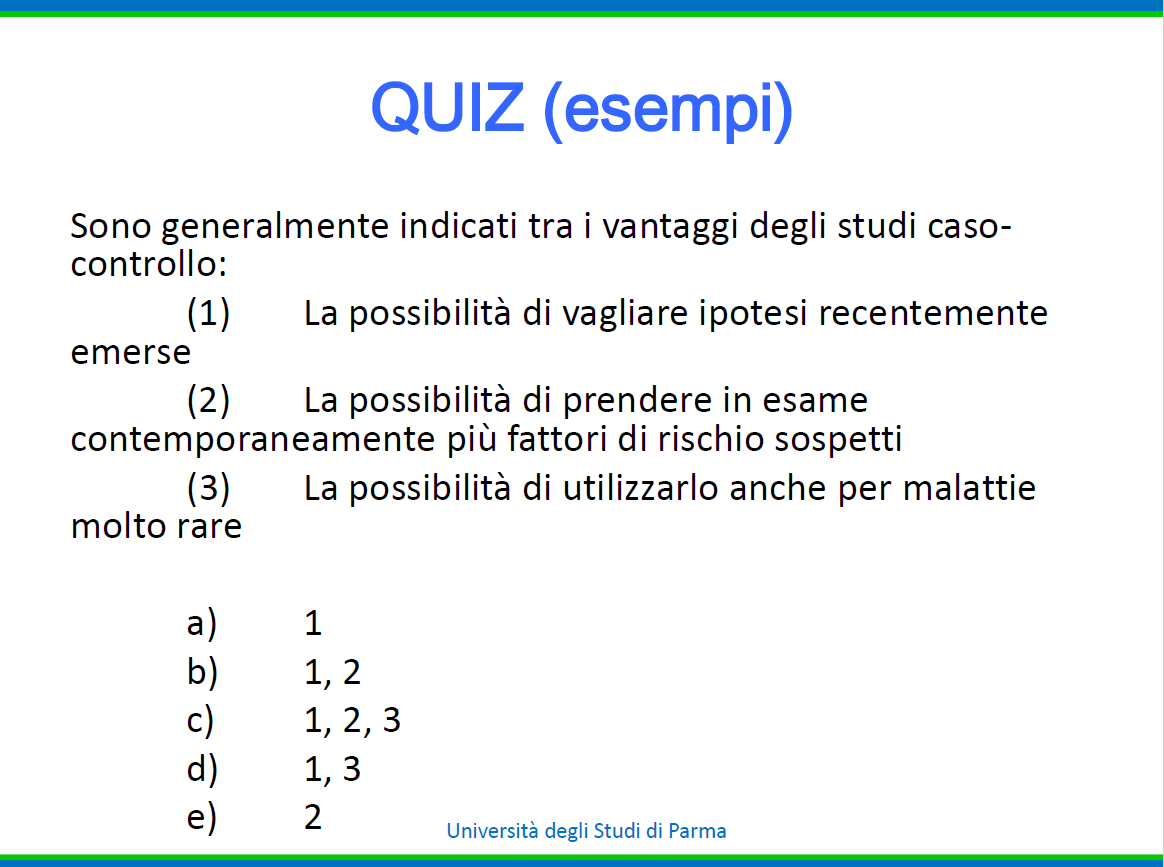
\includegraphics[width=6.21597in,height=4.55417in]{media/image4.emf}

La metà degli incidenti stradali coinvolgono pedoni, ciclisti e
motociclisti, in Europa un po' meno della metà mentre un po' di più in
America. Da questi dati si vede come la bicicletta, mezzo ottimo per la
mobilità sostenibile è in realtà un mezzo abbastanza pericoloso in
termini di incidentalità.

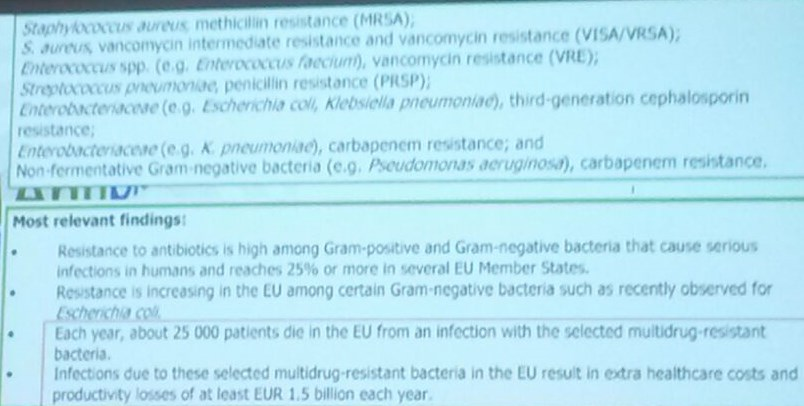
\includegraphics[width=5.62569in,height=4.36250in]{media/image5.emf}~La
mortalità degli incidenti stradali è molto alta e il continente più
colpito è l'Africa mentre il meno colpito è l'Europa. Nel continente
europeo c'è un tasso più alto di mortalità alto in Spagna, Portogallo,
Grecia e Paesi Baltici. C'è un legame stretto tra la mortalità e
condizione stradale infatti dove le strade sono impervie e molto strette
c'è un maggior rischio di incidentalità. I dati europei dal 2001 al 2015
mostrano come i morti si siano dimezzati dal 2001 al 2010 grazie
all'impegno politico generale in questa materia e la EU si è prefissata
come obiettivo di passare da 30.000 a 18.000 morti/morti entro il 2020,
tuttavia il trend discendente si è fermato e quindi serve ancora più
impegno. In Italia il picco degli incidenti si ha nel 2000 e poi anche
qui ha cominciato trend discendente che ha portato da 8000 a 4000
morti/anno con l'obiettivo di arrivare a 1000 morti/anno nel 2020.

Il grosso problema è che la maggior parte dei morti in incidenti
stradali hanno una età giovane, identificando una perdita di anni di
vita molto più alta rispetto a malattie oncologiche o cardiache poiché
queste colpiscono preferenzialmente gli anziani.

Cause d'incidente(Paragrafo)

Oggi si pensa che la principale causa degli incidenti sia l'uso di
dispositivi elettronici come il cellulare. Il problema è che non si
hanno dati su questo perché è molto complicato capire se il soggetto
stava usando o meno il cellulare, più complicato di altri parametri
sempre imputabili ad incidenti come velocità e alcolemia. Tra altri
fattori troviamo la mancata revisione dei veicoli, ormai ridotta come
causa, il trasporto corretto dei bambini o il mancato uso delle cinture
di sicurezza.

Prevenzione (Paragrafo)

La prevenzione si attua con provvedimenti progressivi che interessano la
guida in stato d'ebrezza, limiti di velocità, protezioni per i
motociclisti, ecc... Occorre tener presente che alcune norme sono
efficaci ed altre meno, per esempio: tenere i fari accesi di giorno sia
efficace o meno e in più siamo l'unico paese in EU ad aver imposto
questa cosa, anche perché l'accensione dei fari aumenta il consumo dei
veicoli del 2\%; le rotonde sono un altro mezzo in discussione perché
hanno aumentato gli incidenti ma a fronte di una minore gravità per
l'angolo d'impatto meno pericoloso; se si analizzano i dati dei
seggiolini per bambini si osserva che il rapporto costo-beneficio è
sproporzionato, in quanto il costo è molto alto ma il beneficio che si
guadagna è invece relativamente basso perché chi guida con un bambino a
bordo adotta automaticamente una guida più sicura; infine sui limiti di
velocità c'è del dibattito perché in Germania le autostrade non hanno
limiti e comunque sono tra i paesi con meno incidenti stradali. Tra le
recenti norme, quelle che hanno avuto un miglior impatto invece sono
state la patente a punti e l'abbassamento del limite di alcolemia. La
norma più recente è l'introduzione del omicidio stradale ma non sembra
avere avuto un grande effetto.

Altri fattori di prevenzione derivano dalle caratteristiche dei veicoli
e la presenza di percorsi protetti per pedoni e biciclette. Infine c'è
il potenziamento delle unità di soccorso stradale, dei mezzi pubblici e
l'educazione stradale, estremamente importante in periodo scolastico
perché è il momento dove il bambino interiorizza meglio alcune norme di
Sanità Pubblica.

~

Infortuni domestici (Sottosezione)

Definizione (Paragrafo)

Si definisce come infortunio domestico è \emph{un incidente che presenta
determinate caratteristiche: }

\begin{quote}
•\emph{comporta la compromissione temporanea o definitiva delle
condizioni di salute di una persona, a causa di lesioni di vario tipo}

•\emph{si verifica indipendentemente dalla volontà umana}

•\emph{si verifica in un'abitazione, intesa come l'insieme
dell'appartamento vero e proprio e di eventuali estensioni esterne
(balconi, giardino, garage, cantina, scala ecc).}
\end{quote}

Epidemiologia (Paragrafo)

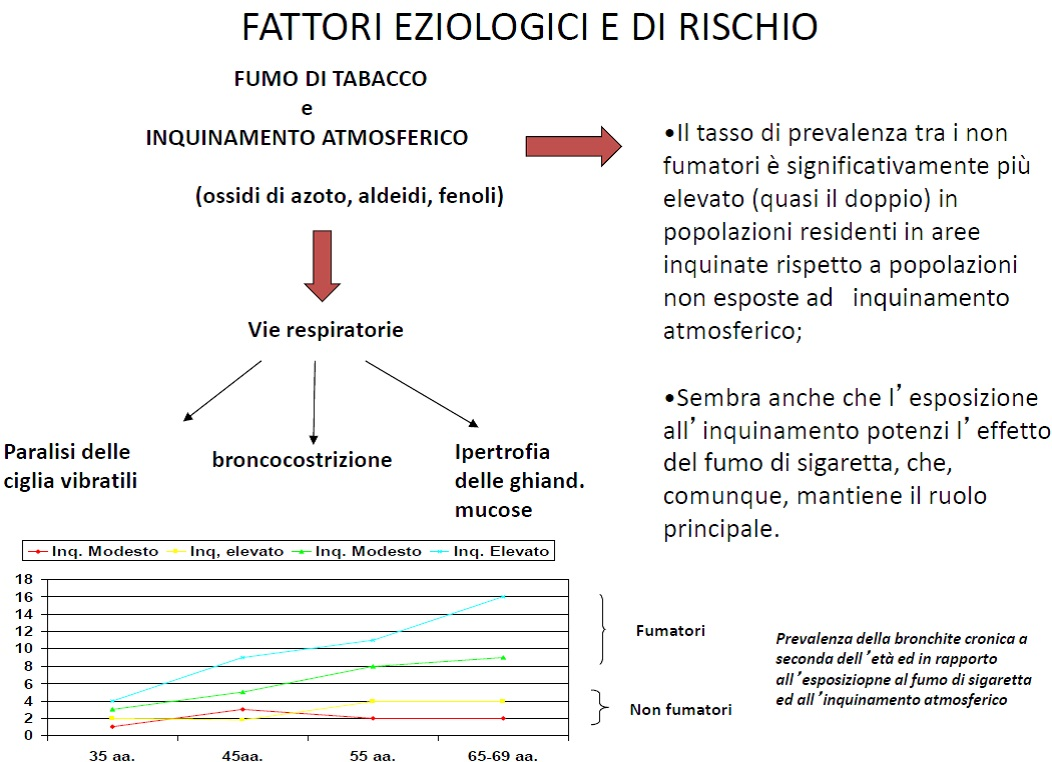
\includegraphics[width=4.69306in,height=3.33472in]{media/image6.emf}

L'incidenza è molto alta, tra le persone intervistate 11\% dichiara un
infortunio domestico nei passati 3 mesi. Le categorie più colpite sono
le donne (perché passano più tempo in casa), gli anziani (a rischio di
danni aggravati dall'osteoporosi) e i neonati. Di gran lunga le più
frequenti sono le cadute e seguono poi gli urti, le ferite, gli
schiacciamenti, le ustioni e gli annegamenti. Tra i luoghi più frequenti
dove si sviluppano troviamo la cucina, il bagno e la camera da letto.
Degli infortunati un 43\% si è recato al PS, 17\% si è recato in un
ambulatorio e 7,9\% è stato ricoverato, questo serve per ricordare che
bisogna tener conto non solo degli effetti sanitari del danno ma anche
l'impatto economico sul Servizio Sanitario.

Prevenzione (Paragrafo)

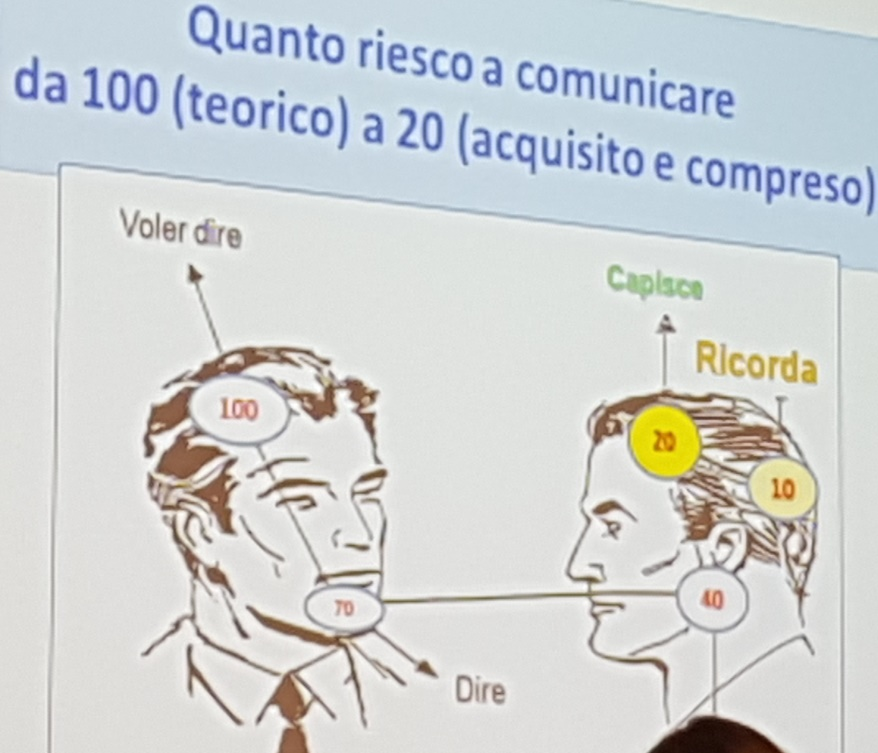
\includegraphics[width=4.94931in,height=3.02014in]{media/image7.emf}

Come in altri campi è possibile fare delle buone raccomandazioni e norme
di sicurezza ma è dovere poi del singolo individuo rispettarle. Se si fa
il caso dei bambini, il 6\% degli incidenti è dovuto ad ingestione di
sostanze tossiche e questo deriva del fatto che il bambino si beve il
detersivo messo del genitore nella bottiglia dell'acqua minerale;
infatti una delle raccomandazioni è quella di non mettere le sostanze
tossiche ad una altezza inferiore di un metro ma non si può fare una
legge che impedisca questa cosa, sta poi al cittadino decidere se
seguire o meno la raccomandazione.

Infortuni sul lavoro(Sottosezione)

Definizione (Paragrafo)

L'infortunio sul lavoro è definito dalla legge come \emph{l'evento, che
avviene per la c.d.~\textbf{causa violenta}, in~\textbf{occasione di
lavoro}~(quindi ricollegabile allo svolgimento dell'attività lavorativa)
dal quale deriva una~\textbf{lesione}~o una~\textbf{malattia}~del corpo
che rende necessaria l'\textbf{astensione dal lavoro~}per~\textbf{più di
tre giorni}.}

Una cosa importante è che nella classificazione degli incidenti sul
lavoro troviamo anche gli incidenti stradali, sia di chi per lavoro
guida i veicoli sia chi guida per arrivare da casa alle sede di lavoro.
Questo crea un po' di confusione per la sovrapposizione tra incidenti
sul lavoro ed incidenti stradali ma serve perché il lavoratore sia
assicurato dal momento che si reca alla sede di lavoro.

Epidemiologia (Paragrafo)


\includegraphics[width=4.58333in,height=3.05903in]{media/image8.emf}

I settori lavorativi più a rischio sono il settore agricolo,
considerando anche il basso numero di personale impiegato, il settore
industriale, con particolare riguardo all'edilizia, ai trasporti e alla
attività estrattiva. Dai dati americani al primo posto troviamo i
pescatori, non è molto chiaro ancora il motivo, poi taglialegna, quindi
gli addetti agli smaltimento dei rifiuti, in misura meno grave, e quindi
le solite classi citate prima, agricoltori ecc...

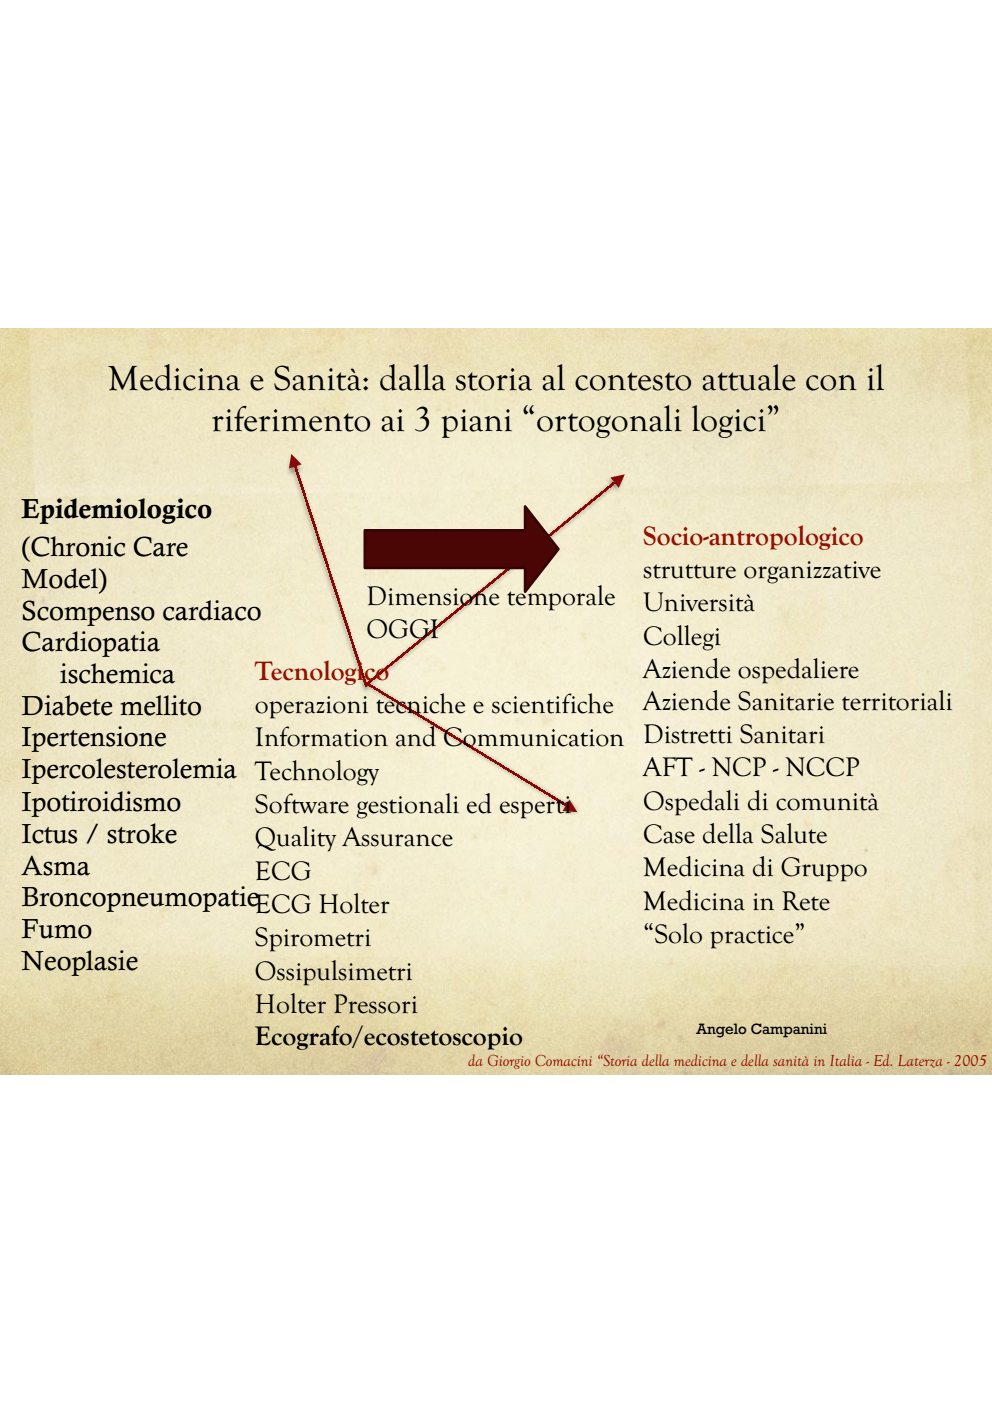
\includegraphics[width=3.34931in,height=2.38194in]{media/image9.emf}

La mortalità ha un primo picco tra i 15-24 anni e poi un trend crescente
per età dai 30-40 anni per arrivare ai picchi dopo i 65 anni.

Prevenzione (Paragrafo)

La prevenzione si attua mediante la raccolta dei dati e le misure
legislative dal decreto 626 del '94, prima normativa sulla sicurezza del
lavoro, e ripreso da un testo unico del 2008 e modificato nel 2009. qui
c'è un concetto importante, ossia che responsabilità della sicurezza dei
lavoratori è in capo al datore di lavoro. Nel caso dell'Università di
Medicina gli studenti sono equiparati a lavoratori e non a caso al primo
anno si fa un corso di sicurezza sul lavoro, per istruire a quali sono i
rischi come cattiva postura o rischio biologico. Tutti i datori di
lavoro devono produrre un documento per la valutazione del rischio e,
dove necessario, adottare tutte le misure precauzionali o preventive per
la salute del lavoratore. Oltre al datore di lavoro, altre figure chiave
sono il responsabile per la sicurezza, il medico competente che svolge
visite periodiche e di assunzione del lavoratore, il responsabile del
servizio prevenzione e protezione e un rappresentante dei lavoratori per
la sicurezza ogni 40 -- 50 lavoratori. Tuttavia anche se il testo unico
prevede norme formali che hanno permesso una riduzione dell'incidenza di
infortuni ci sono ancora problemi per sacche incontrollate che si
identificano sostanzialmente con il lavoro in nero che sfugge ai dati
generali.

Mobbing (Paragrafo)

Il Mobbing è \emph{una sistematica persecuzione esercitata sul posto di
lavoro da colleghi o superiori nei confronti di un individuo,
consistente per lo più in piccoli atti quotidiani di emarginazione
sociale, violenza psicologica o sabotaggio professionale, ma che può
spingersi fino all'aggressione fisica.} Questo che frequentemente
disagio ai lavoratori e per questo chi ne è vittima deve essere tutelato
e per questo in Italia c'è una sentenza. Per prevenire il fenomeno è
necesserio conoscerlo, migliorare le condizioni lavorative e dove
necessario creare comitati per la tutela del mobbing che ricevono le
denunce e prendono provvedimenti.

Burn out (Paragrafo)

riguarda lo stress di operatori che svolgono attività alienanti,
ripetitive o particolarmente delicate che portano un deterioramento
dell'impegno e delle emozione con problemi di adattamento tra persona e
lavoro. Non è strano quindi che la terapia consiste nell'allontanamento
del soggetto per un po' di tempo dal lavoro. Tra le figure a rischio in
medicina troviamo soprattutto l'anestesista e alcune chirurgie. La
prevenzione consiste ne gestire le cause, dare supporto psicologico,
dormire e svolgere attività fisica regolarmente.

\end{document}
